\documentclass[a4,12pt]{scrartcl}

%Basic 
\usepackage[utf8]{inputenc}
\usepackage[ngerman]{babel}
\usepackage[T1]{fontenc}
%Schrift 
%\usepackage{fontspec} 
%\setmainfont{Arial} 
%Zeilenabstand
\usepackage{setspace}
\setstretch {1.3}
\usepackage{float}
\usepackage[bottom = 3.50cm]{geometry}

%Titel Seite
\usepackage{titling} %Wird benötigt damit \maketitle die Variabeln title, author und date nicht überschreibt
\title{Test Cases}
\subtitle{Projekt: software name}
\author{David Meister \and Andreas Stalder}		
 %mit /and können Personen hinzugefügt werden
\date{\today}


%Kopf, Fusszeile
\usepackage{fancyhdr}
\pagestyle{fancy}
\lhead{}
\chead{}
\rhead{software name}
\lfoot{\thetitle \: v1.0 }
\cfoot{\today }
\rfoot{Seite \thepage}
\renewcommand{\headrulewidth}{0.4pt}

%Bilder
\usepackage{graphicx}

%Zeichnen
\usepackage{tikz}

%Tabellen
\usepackage{booktabs}
\usepackage{longtable}

%Codesnippets
\usepackage{listings}
\lstset{language=java,basicstyle=\footnotesize,frame=single} %backgroundcolor=\color{lightgray}

%Querformat für eine Seite
\usepackage{lscape}
\usepackage{rotating}
\usepackage{pdflscape}

%URL 
\usepackage[colorlinks=true, linkcolor=blue, urlcolor=blue, citecolor=blue]{hyperref}
\urlstyle{same} 


%Loremimpsum
\usepackage{lipsum}



\begin{document}

%\clearpage\maketitle
\begin{titlepage}
	\centering
	\vspace{5cm}
	\begin{center}
%	\includegraphics[width=0.50\textwidth]{}
	\end{center}
	{\huge\bfseries software name\par}
	\vspace{8cm}
	\raggedright
	{\bfseries HSR Studienarbeit Network Unit Testing\par}
	{\huge\bfseries Network testing\par}
	\vspace{1cm}
	{\theauthor \par}
	{\today\par}

\end{titlepage}

\section{Änderungsgeschichte}

\begin{table}[htb]
\centering
    \begin{tabular}{@{} l l l l@{}}\toprule    
    {Datum} & {Version} & {Änderung} & {Autor}\\ \midrule
    27.09.16 & 1.0 & Erstellung erster Version & dm/as\\ \addlinespace
    \end{tabular}
\caption{\textbf{Änderungsgeschichte}}
\end{table}

\newpage

%\thispagestyle{empty}
\tableofcontents
\newpage


\section{Einführung}
\subsection{Zweck}
Dieses Dokument stellt den Projektplan für unser Studienarbeit dar, es dient zur Planung, Steuerung und Kontrolle.
\subsection{Gültigkeitsbereich}
Dieses Dokument ist über die gesamte Projektdauer gültig. Es wird in späteren Iterationen angepasst. Somit ist jeweils die neuste Version des Dokuments gültig und alte Versionen sind obsolet.
\subsection{Referenzen}
\begin{description}
Noch keine.
%  \item[jNetPcap] \hfill \\
%  \url{http://jnetpcap.com/}
\end{description}

\section{Einleitung}
\subsection{Testing Motivation}
\subsection{}

\section{Device Tests}
\subsection{Scope}
\subsection{Nutzen}
\subsection{Beispiele von Test Cases}
\newpage
\section{Circuit Tests}
\subsection{Scope}
Mit Circuit Tests möchte man die Verbindungen der Devices testen. Mögliche LAN Devices sind unter anderem Access-, Distribution-, und Core Switches, aber auch Router oder Firewalls. Denkbar sind auch Verbindungen im WAN Bereich, ob Ethernet, ATM oder MPLS. Diese Devices haben jeweils unterschiedliche Verbindungen zueinander. Circuit Tests überprüfen Anhand verschiedener Bewertungskriterien die Qualität und Charakteristika dieser Verbindungen.\\

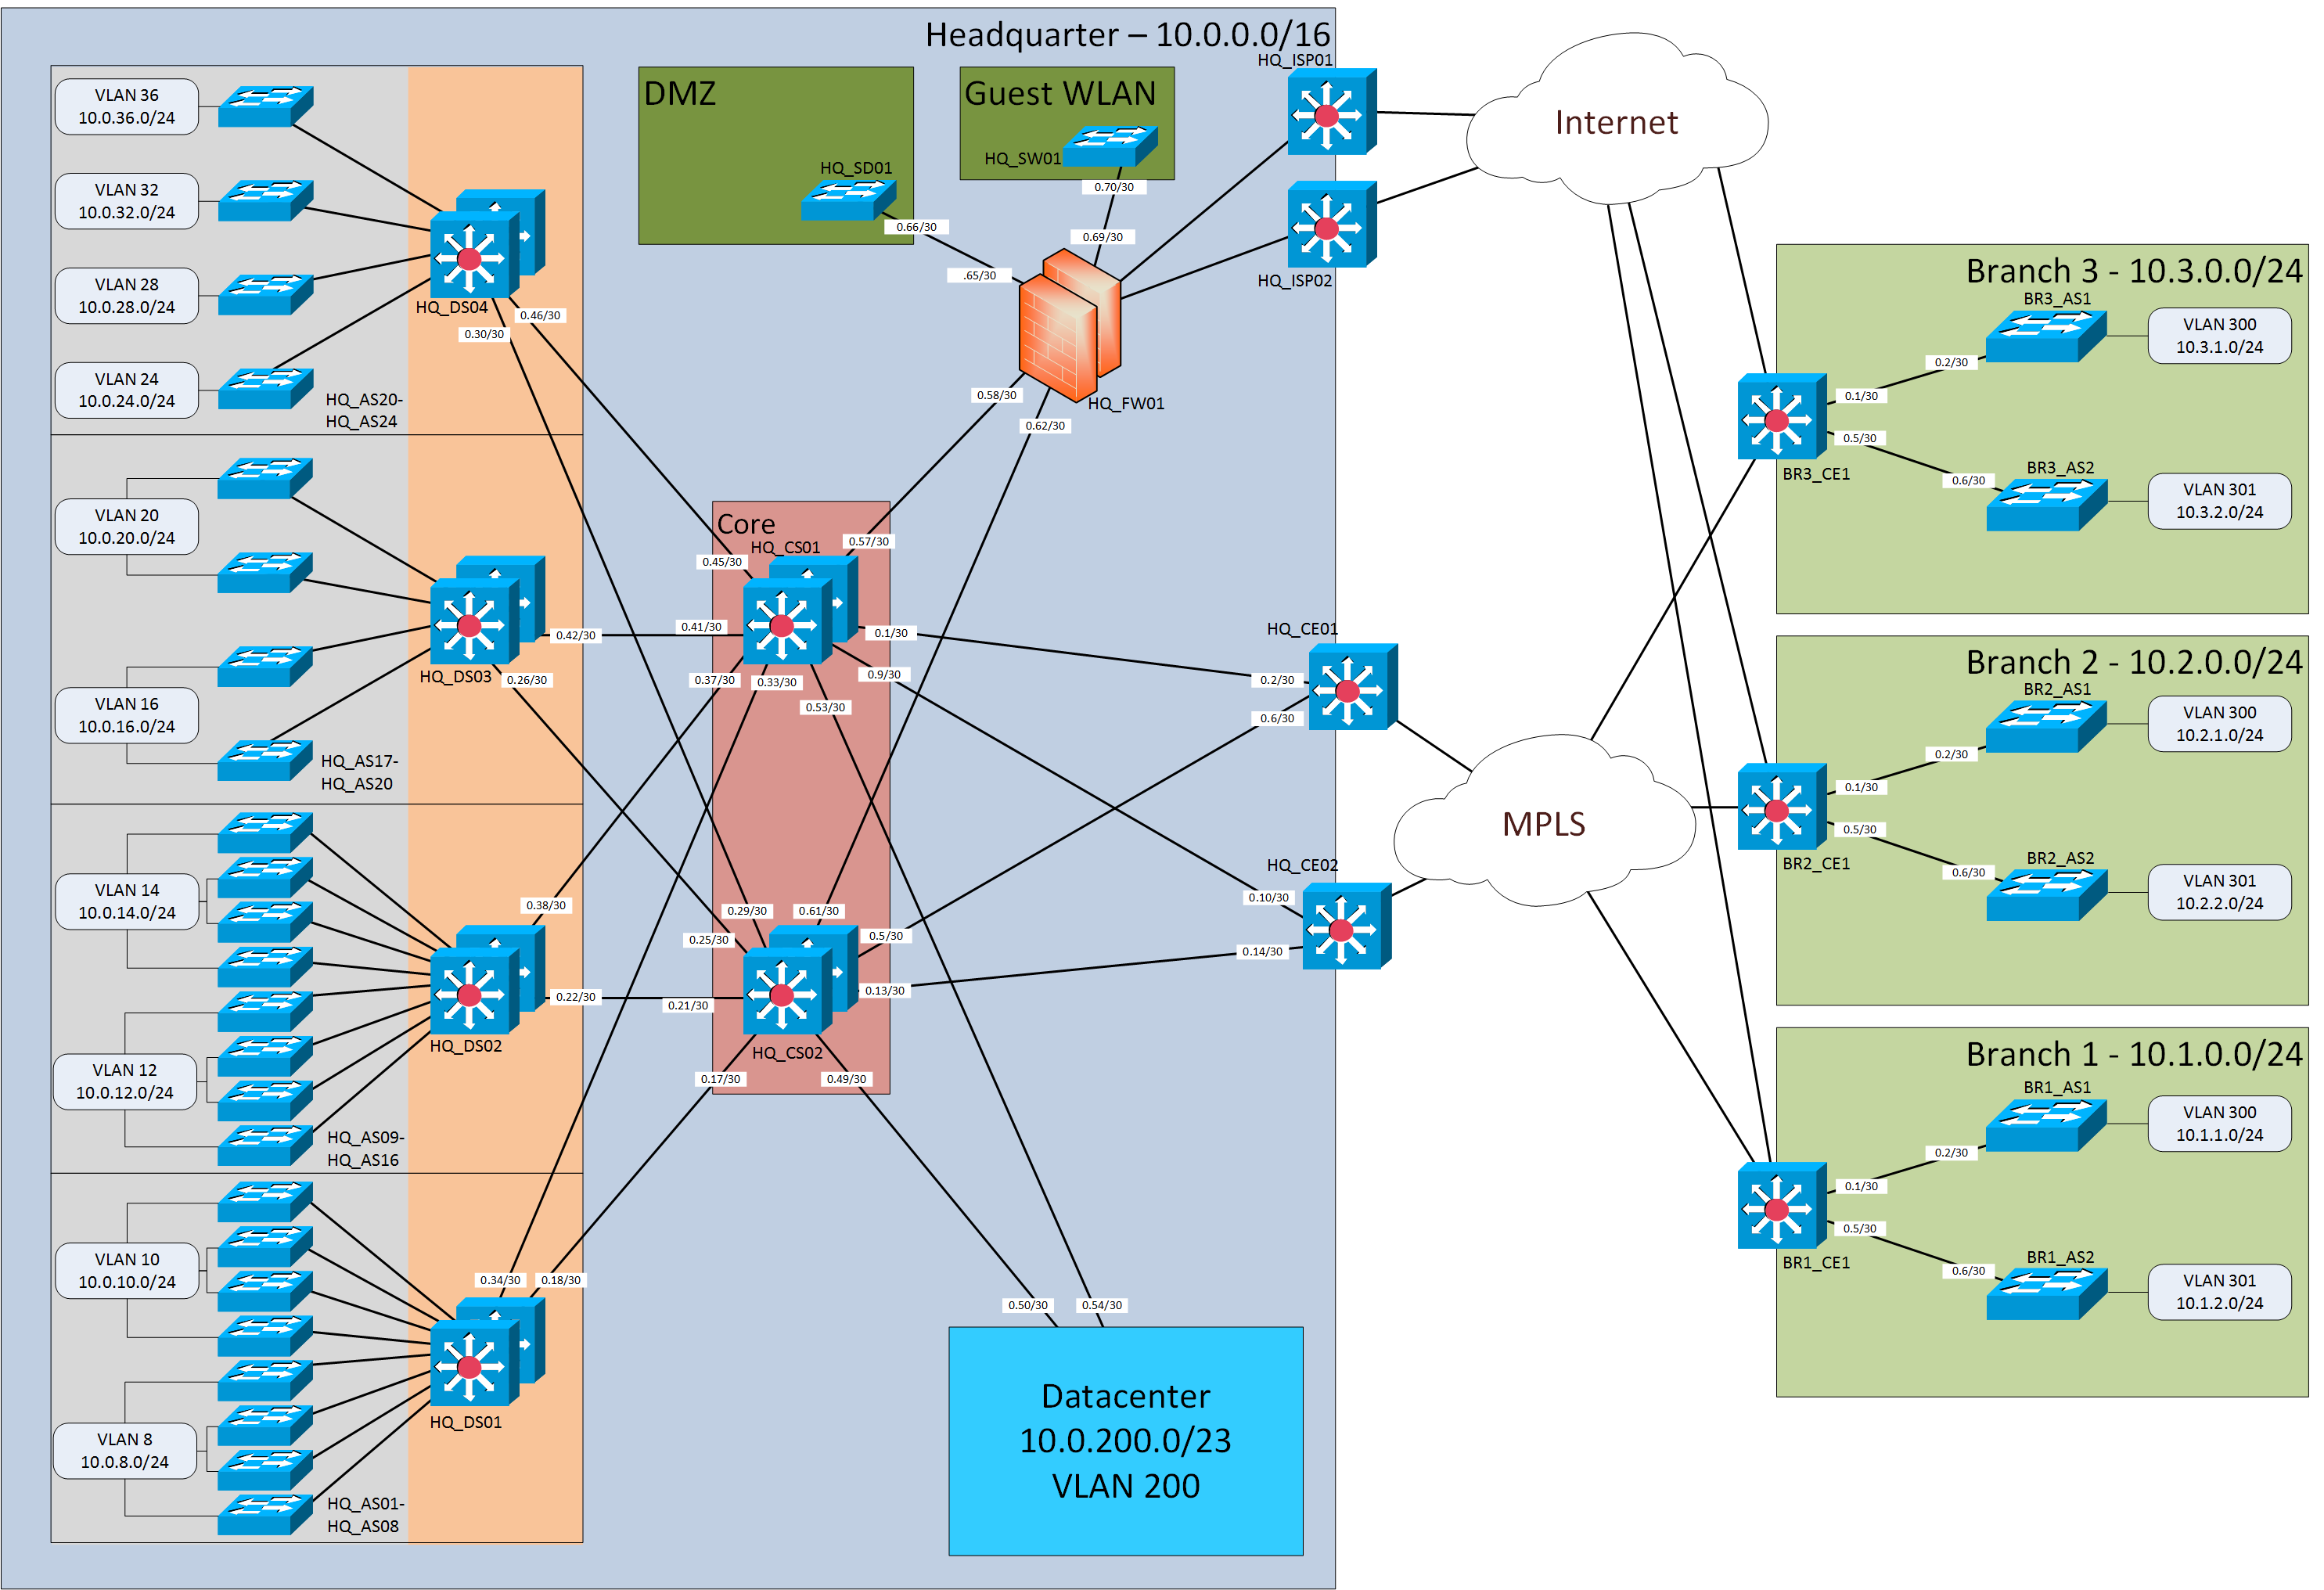
\includegraphics[width=1\textwidth]{figures/Netzwerk_logisch.png}\\

\noindent Wenn von Verbindungsqualität gesprochen wird, möchte man vor allem bestimmte Verbindungsspezifische Parameter wie Round Trip Times, Jitter, Throughput Packet Loss testen. Je nach Verbindung, welche es zu testen gilt, kann man sinnvolle Grenzwerte festlegen. So können gewisse Throughput Werte auf der WAN Verbindung einer Firewall akzeptabel sein, während derselbe Wert auf der LAN Verbindung zu niedrig wäre.\\

\noindent Typischerweise bewegt man sich bei Circuit Tests auf den OSI-Layern 1-3. Es muss jeweils überlegt werden, welche Tests sinnvoll sind, um die komplette Funktionalität der Verbindung auf unterschiedlichen Test Cases abzubilden.   
\subsection{Nutzen}
Durch systematisches Testen der Verbindungen gewinnen wir Vertrauen in die Funktionalität der Verbindungen. Changes im Netzwerk, seien es einfache Konfigurationsänderungen, oder Austausch eines oder mehrerer Devices, können bei auftretenden Fehlern schwerwiegende Folgen mit sich bringen.\\

\noindent Als Verantwortlicher Netzwerk Engineer trägt man eine grosse Verantwortung. Beim unsystematischen ad-hoc Testing werden leider oft essenzielle Funktionen und Parameter nicht getestet. Es wird sich ganz auf das Know-How und die Erfahrung des Verantwortlichen Engineers gestützt. Unter Zeitdruck werden oft nur sehr wenige Tests durchgeführt, bis das Netzwerk wieder für den produktiven Betrieb freigegeben wird. Mit systematischen Circuit Tests werden beispielsweise fehlende Links und Verbindungsfehler auf allen Devices schnell erkannt. 
\subsection{Beispiele von Test Cases}
\subsubsection{Round Trip Time}
Bei der Round Trip Time (RTT) möchte man herausfinden, wieviel Zeit für die Übertragung und Verarbeitung eines Datenpakets über die Verbindung benötigt wird. Da bei den Circuit Tests keine high-level Services getestet werden, sollen Datenpakete gesendet werden, für welche die Gegenstation extrem wenig Zeit benötigt, um diese zu Verarbeiten. Das Interesse besteht also hauptsächlich in der benötigten Zeit für den Übertragungsweg.\\

\noindent Der bekannteste Weg, um die RTT zu ermitteln, ist der ping-Befehl, welcher einen ICMP Request auslöst. Mit Ping kann man die RTT innerhalb der Broadcast Domain, aber auch über dessen Grenzen hinweg ins gesamte Internet herausfinden. Es gibt jedoch noch andere Wege, um die RTT zu bestimmen. Mittels arping wird die RTT über ARP Pakete bestimmt, oder über httping wird die Antwortzeit über das HTTP Protokoll ermittelt. Für Circuit Tests scheint der 'normale' ping über ICMP jedoch der sinnvollste.\\

\noindent Bei der RTT gilt es zu beachten, dass bei zwei Devices $\{a,b\}$ die benötigte Übertragungszeit von a$\rightarrow$b $\neq$ b$\rightarrow$a sein kann. Beim Circuit Testing ist aber eher unwahrscheinlich, dass sich die Latenzzeit der beiden Übertragungswege gross unterscheiden, da in aller Regel in derselben Broadcastdomain oder über sehr wenige Hops getestet wird.\\

\noindent Mögliche Einflussgrössen der RTT sind die Distanz, verwendete Kabel, Routing/Switching processing, Queueing Delay oder mögliche Übertragungsfehler.
\subsubsection{}  
\section{Routing Tests}
\subsection{Scope}
\subsection{Nutzen}
\subsection{Beispiele von Test Cases}






\section{Traffic Tests}
\subsection{Scope}
\subsection{Nutzen}
\subsection{Beispiele von Test Cases}
\subsubsection{QoS}
\subsubsection{Throughput}
Throughput ist ein wichtiger Punkt im Bereich Netzwerktest. Hier gibt es zwei Möglichkeiten. Den Link-Throughput, sowie den End-to-End-Throughput.
\minisec{Link-Throughput}
Beim Link-Throughput wird der Layer 2 durchsatz gemessen. 
\minisec{End-to-End-Throughput}



\section{Application Tests}
\subsection{Scope}
Mit den Application Tests, werden Netzwerkservices getestet. Diese können zum Beispiel DNS, DHCP, Webservice usw. sein.
Um sicherzustellen, damit bei einer Firewallumstellung alle Service noch funktionieren, schickt man Anfragen an die Services.
\subsection{Nutzen}
So kann man sicherstellen, dass alle Komponenten noch korrekt miteinander kommunizieren und das nichts geblockt wird.

\subsection{Beispiele von Test Cases}
\subsubsection{DNS}

\subsubsection{DHCP}

\subsubsection{Webservice}
Ein Webservice kann sehr leicht getestet werden. Man kann dem Server eine Anfragen mit senden und weiss was die Antwort sein muss.
Beispiel anfragen sind: \newline
- GET www.example.com/index.html HTTP/1.1 \newline
- GET www.example.com/user/12 HTTP/1.1 \newline
\newline
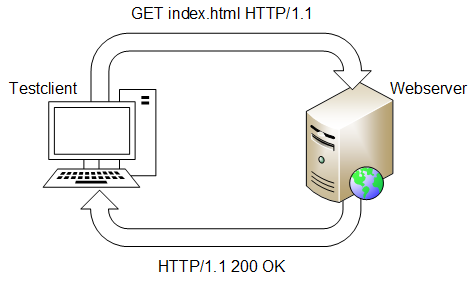
\includegraphics[scale=1]{figures/httpget.png}

\subsubsection{SSH}

\end{document}

